\documentclass[a4paper, twocolumn]{article}

% font handling
\usepackage{fontspec}

% uncomment (or change) if you don't have this particular font installed
\setmainfont{Palatino Linotype}

% for setting the linespace (\setstretch)
\usepackage{setspace}

% distance between the columns
\setlength{\columnsep}{1cm}

% for compactitem
\usepackage{paralist}

% for comments
\usepackage{verbatim}

\usepackage[
	sorting=none,
	minbibnames=8,
	maxbibnames=9,
	block=space,
	backend=biber
]{biblatex}
\bibliography{bibliography}

\usepackage{lipsum}

\begin{document}

%=============================
{
	\parindent0pt
	\setstretch{1.4}
	\ \\ \ \\ \ \\

	\hrulefill
	\vspace{0.0cm}
	\begin{spacing}{2.1}
	{	
		\flushleft
		\fontsize{22pt}{44pt}\selectfont 
		Donec Vehicula Augue eu Neque Esuada Fames 
	}\\
	\textsc{Master's Thesis Proposal}
	\end{spacing}

	\ \\ \ \\
	{
		\setstretch{1.2}
		Michael M\"uller\\
		michi@uni-ulm.de\\
		Institute of Distributed Systems\\
		Ulm University\par
	}
	\ \\

	\hrulefill

}

{
	\setstretch{1.1}
	In dieser Arbeit wird der DYCOS-Algorithmus, wie er in \cite{aggarwal2011}
vorgestellt wurde, erklärt. Er arbeitet auf Graphen, deren Knoten teilweise mit
Beschriftungen versehen sind und ergänzt automatisch Beschriftungen für Knoten,
die bisher noch keine Beschriftung haben. Dieser Vorgang wird
\enquote{Klassifizierung} genannt. Dazu verwendet er die Struktur des Graphen
sowie textuelle Informationen, die den Knoten zugeordnet sind. Die in
\cite{aggarwal2011} beschriebene experimentelle Analyse ergab, dass er auch auf
dynamischen Graphen mit 19\,396 bzw. 806\,635 Knoten, von denen nur
14\,814 bzw. 18\,999 beschriftet waren, innerhalb von weniger als
einer Minute auf einem Kern einer Intel Xeon 2.5\,GHz~CPU mit 32\,G~RAM
ausgeführt werden kann.\\
Zusätzlich wird \cite{aggarwal2011} kritisch Erörtert und und es werden
mögliche Erweiterungen des DYCOS-Algorithmus vorgeschlagen.

\textbf{Keywords:} DYCOS, Label Propagation, Knotenklassifizierung

}
\newpage

%=============================
%!TEX root = Sommerakademie-2015-Forschung.tex
\section{Einleitung}
\subsection{Was ist On-Line Recognition?}

\begin{frame}{Demo}
    \begin{figure}[h]
        \centering
        \includegraphics*[width=0.7\linewidth, keepaspectratio]{images/Classification.png}
    \end{figure}

    \href{http://write-math.com}{write-math.com}
\end{frame}

\begin{frame}{Was ist On-Line Recognition?}
\medskip
\begin{columns}[t,onlytextwidth]
\begin{column}{.5\textwidth}
{\Large Off-line Recognition}
\begin{figure}[h]
    \centering
    \includegraphics*[width=0.7\linewidth, keepaspectratio]{images/A-pixel.png}
\end{figure}
\end{column}
\begin{column}{.5\textwidth}
{\Large On-line Recognition}
\begin{figure}[h]
    \centering
    \includegraphics*[width=0.7\linewidth, keepaspectratio]{images/A-vektor.png}
\end{figure}
\end{column}
\end{columns}
\end{frame}

\begin{frame}{Was wollen wir?}
    \[f(\text{Merkmale}) = \begin{pmatrix}0.7\\ 0.1\\ 0.2\end{pmatrix} = \begin{pmatrix} \mathbb{P}(\gamma)\\ \mathbb{P}(\text{ö})\\ \mathbb{P}(\heartsuit) \end{pmatrix}\]
    \medskip
    \visible<2->{
        \begin{center}
        {\Large Gesucht: Funktion $f$}\\
        (und Merkmalsextraktion)
    }
    \end{center}
\end{frame}

\begin{frame}{Merkmalsextraktion}
    \begin{figure}[h]
        \centering
        \includegraphics*[width=0.7\linewidth, keepaspectratio]{images/A-vektor-merkmalsbildung.png}
    \end{figure}

    Merkmalsvektor fester Länge ist praktisch
\end{frame}

\section{Funktionen}
\subsection{Funktionen}

\begin{frame}{Funktionen}
\begin{figure}[h]
    \centering
    \includegraphics*[width=0.7\linewidth, keepaspectratio]{images/function-machine.png}
\end{figure}
\end{frame}
\begin{frame}{Funktionen}
    \medskip
    \begin{columns}[t,onlytextwidth]
    \begin{column}{.5\textwidth}{
        \begin{itemize}[<+->]
            \item $f(x) = x^2$ ist $f: \mathbb{R} \rightarrow \mathbb{R}$
            \item $f(x, y) = x^2 + y^2$ ist $f: \mathbb{R}^2 \rightarrow \mathbb{R}$
            \item $f(x, y) = (x^2 + y^2, x \cdot y)$ ist $f: \mathbb{R}^2 \rightarrow \mathbb{R}^2$
        \end{itemize}
    }
    \end{column}
    \begin{column}{.4\textwidth}
    \only<1>{
        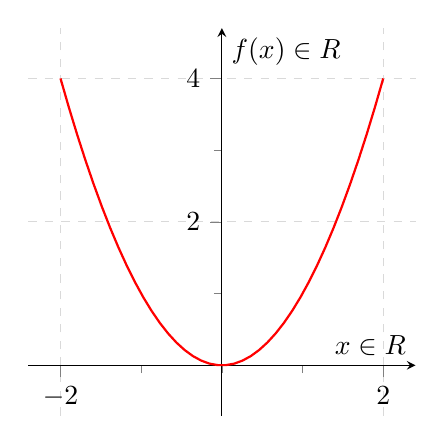
\begin{tikzpicture}
            \begin{axis}[
                legend pos=south west,
                axis x line=middle,
                axis y line=middle,
                grid = major,
                width=6.5cm,
                height=6.5cm,
                grid style={dashed, gray!30},
                xmin=-2,     % start the diagram at this x-coordinate
                xmax= 2,     % end   the diagram at this x-coordinate
                ymin=-0.25,  % start the diagram at this y-coordinate
                ymax= 4.25,  % end   the diagram at this y-coordinate
                axis background/.style={fill=white},
                xlabel=$x \in \mathbb{R}$,
                ylabel=$f(x) \in \mathbb{R}$,
                %xticklabels={-2,-1.6,...,7},
                %yticklabels={-8,-7,...,8},
                tick align=outside,
                minor tick num=-3,
                enlargelimits=true,
                tension=0.08]
              \addplot[domain=-2:2, red, thick,samples=40] {x*x};
            \end{axis}
        \end{tikzpicture}
    }
    \only<2->{
        \pgfplotsset{
            colormap={whitered}{
                color(0cm)=(white);
                color(1cm)=(orange!75!red)
            }
        }
        \begin{tikzpicture}
            \begin{axis}[
            colormap name=whitered,
            width=5.5cm,
            height=5.5cm,
            view={340}{25},
            enlargelimits=false,
            grid=major,
            domain=-3:3,
            y domain=-3:3,
            samples=56, %57 : TeX capacity exceeded, sorry [main memory size=3000000].
                        % see also http://tex.stackexchange.com/a/7954/5645
            xlabel=$x$,
            ylabel=$y$,
            zlabel={$f(x,y)$},
            ]
              \addplot3[surf] {x^2 + y^2};
            \end{axis}
        \end{tikzpicture}
    }
    \end{column}
    \end{columns}
\end{frame}

\begin{frame}{Funktionen mit Parametern}
    \begin{columns}
    \begin{column}{.5\textwidth}
        {\Large Mit Parametern}
        \begin{itemize}[<+->]
            \item $f(x) = x^2$
            \item $f(x) = 2 \cdot x^2$
            \item $f(x) = \nicefrac{1}{2} \cdot x^2$
            \item $f(x) = a \cdot x^2$
            \item $f(x_1, \dots, x_{166}) = \sum_{i=1}^{166} a_i \cdot x_i$\\
                  $\mathbb{R}^{166} \rightarrow \mathbb{R}$
            \item $f(x_1, \dots, x_{166}) = (\sum_{i=1}^{166} a_i \cdot x_i, \dots, \sum_{i=1}^{166} z_i \cdot x_i)$\\
                  $\mathbb{R}^{166} \rightarrow \mathbb{R}^{\text(\# Klassen)}$
        \end{itemize}
    \end{column}
    \begin{column}{.4\textwidth}
        \begin{tikzpicture}
            \begin{axis}[
                legend pos=south west,
                axis x line=middle,
                axis y line=middle,
                grid = major,
                width=6.5cm,
                height=6.5cm,
                grid style={dashed, gray!30},
                xmin=-2,     % start the diagram at this x-coordinate
                xmax= 2,     % end   the diagram at this x-coordinate
                ymin=-0.25,  % start the diagram at this y-coordinate
                ymax= 4.25,  % end   the diagram at this y-coordinate
                axis background/.style={fill=white},
                xlabel=$x \in \mathbb{R}$,
                ylabel=$f(x) \in \mathbb{R}$,
                %xticklabels={-2,-1.6,...,7},
                %yticklabels={-8,-7,...,8},
                tick align=outside,
                minor tick num=-3,
                enlargelimits=true,
                tension=0.08]
              \only<1->{\addplot[domain=-2:2, red, thick,samples=40] {x*x};}
              \only<2->{\addplot[domain=-2:2, blue, thick,samples=40] {2*x*x};}
              \only<3->{\addplot[domain=-2:2, green, thick,samples=40] {0.5*x*x};}
            \end{axis}
        \end{tikzpicture}
    \end{column}
    \end{columns}
\end{frame}

\begin{frame}{Fehlerfunktion}
    \begin{itemize}[<+->]
        \item \textbf{Daten $(x_{i,1}, \dots, x_{i,n}, y_{i,1}, \dots, y_{i,\text{\# Klassen}})$}: Beispiele für den Computer
        \item \textbf{Aktuelles Modell $f$}: Funktion mit vielen Parametern
        \item \textbf{Fehlerfunktion}: Wie gut ist $f$ für die vorhandenen
              Daten?
    \end{itemize}
\end{frame}

\begin{frame}{Fehlerfunktion}
    Abbildung von \textbf{Parameterraum} auf den Fehler ($\mathbb{R}_0^+$)
\end{frame}

\begin{frame}{Minimieren mit Ableitungen}
    \begin{figure}[h]
        \centering
        \includegraphics*[width=0.7\linewidth, keepaspectratio]{images/derivative-function.png}
    \end{figure}
\end{frame}

\begin{frame}{Gradientenabstieg}
    \begin{figure}[h]
        \centering
        \includegraphics*[width=0.7\linewidth, keepaspectratio]{images/gradient-descent.png}
    \end{figure}
\end{frame}


\section{Neuronale Netze}
\subsection{Neuronale Netze}
\begin{frame}{Neuronale Netze}{}
    \begin{itemize}[<+->]
        \item Menge von parametrisierten Funktionen
              $\mathbb{R}^n \rightarrow \mathbb{R}^{\text(\# Klassen)}$
        \item $\mathbb{R}^n$: Eingabe,\\z.B. Farbe von Pixel~1, Farbe von Pixel~2, \dots
        \item $\mathbb{R}^{\text(\# Klassen)}$: Ausgabe,\\Wahrscheinlichkeit der Klasse (z.B. 0, 1, 2, 3, 4, 5, 6, 7, 8, 9)
        \item Ableitbar
    \end{itemize}
\end{frame}

\section{Ausblick}
\subsection{Ausblick}
\begin{frame}{Ausblick}
    Erkennung von Formeln
    \begin{itemize}[<+->]
        \item Aufbau eines Sprachmodells der Mathematik
        \item Erweiterung der Symboldatenbank
        \item Segmentierung
    \end{itemize}
\end{frame}


\section{System Model}
\label{sec:system-model}

\subsection{Concept}
\lipsum[1]

\begin{compactitem}
	\item \lipsum[53]
	\item \lipsum[11]
\end{compactitem}

\lipsum[43]

\subsection{Implementation}
\lipsum[2]

\section{Conclusion}
\label{sec:conclusion}

\lipsum[9-10]


\section{References}
% the \nocite command leads to the whole bibliography
% being displayed (without any \cite commands necessary).
% remove this command in order to get the "normal" behavior.
\nocite{*}
\printbibliography[heading=none]

\end{document}
